\chapter{Πειραματική Αξιολόγηση}
\label{ch:Experimental Evaluation}
Οι διάφορες υλοποιήσεις που πραγματοποιήθηκαν στα πλαίσια της τρέχουσας διπλωματικής εργασίας αξιολογήθηκαν πειραματικά με τη χρήση μετροπρογραμμάτων (benchmarks) τόσο για την επιβεβαίωση της ορθότητας της υλοποίησης, όσο και για τη μέτρηση των επιδόσεων που επιτεύχθηκαν.


\section{Περιγραφή Συστημάτων}
\label{sec:Systems Description}
Η εκτέλεση των πειραμάτων έγινε σε υπολογιστικά συστήματα που εκπροσωπούν διαδεδομένες και ενδιαφέρουσες αρχιτεκτονικές οργανώσεις, όπως για παράδειγμα συστήματα τύπου SMP και NUMA. Τα χαρακτηριστικά των συστημάτων αυτών, τόσο από άποψη υλικού, όσο και από άποψη λογισμικού, φαίνονται στους Πίνακες \ref{tab:exp-systems-hardware} και \ref{tab:exp-systems-software}. Η αρχιτεκτονική των επεξεργαστών όλων των συστημάτων είναι η \textit{x86-64} ενώ το μέγεθος μιας γραμμής της κρυφής μνήμης είναι 64 bytes.

Οι μεταφραστές οι οποίοι χρησιμοποιήθηκαν για τη συγκριτική αξιολόγηση του μεταφραστή OMPi είναι ο \textit{GNU C Compiler} (GCC), ο \textit{Intel C Compiler} (ICC)\footnote{Εγκαταστάθηκε μέσω των oneAPI Toolkits της Intel\textsuperscript{\textregistered}.} και ο \textit{Clang}. Ο πηγαίος κώδικας του OMPi μεταφράστηκε με τον GCC, ενώ τα απαιτούμενα πακέτα λογισμικού είναι διαθέσιμα στο Παράρτημα \ref{app:OMPi's software requirements}.

\begin{table}
	\centering
		\begin{tabular}{|c||c|c|c|c|c|c|}
		\hline
		Hostname & Proc. Mfr. & NUMA nodes & Sockets & Cores & H/W threads & RAM \\
		\hline \hline
		\texttt{parade} & Intel & 4 & 4 & 64 & 128 & 256 GB \\
		\hline
		\texttt{paragon} & AMD  & 4 & 2 & 24 & 24 & 16 GB \\
		\hline
		\texttt{opti3060} & Intel & 1 & 1 & 4 & 4 & 8 GB \\
		\hline
		\texttt{ideapad} & Intel & 1 & 1 & 2 & 4 & 8 GB \\
		\hline
		\end{tabular}
		\caption{Χαρακτηριστικά υλικού των πειραματικών συστημάτων.}
		\label{tab:exp-systems-hardware}
\end{table}

\begin{table}
	\centering
		\begin{tabular}{|c||c|c|c|c|c|c|c|}
		\hline
		Hostname & OS & GCC & ICC & Clang & hwloc & Linux kernel \\
		\hline \hline
		\texttt{parade} & CentOS 8 & \texttt{8.4.1} & \texttt{2021.3.0} & \texttt{11.0.0} & \texttt{2.2.0} & \texttt{4.18.0} \\
		\hline
		\texttt{paragon} & CentOS 8 & \texttt{8.4.1} & \texttt{2021.3.0} & \texttt{11.0.0} & \texttt{2.2.0} & \texttt{4.18.0} \\
		\hline
		\texttt{opti3060} & Ubuntu 18.04.3 & \texttt{7.5.0} & \texttt{N/A} & \texttt{N/A} & \texttt{1.11.9} & \texttt{5.0.0} \\
		\hline
		\texttt{ideapad} & Mint 20.2 & \texttt{9.3.0} & \texttt{2021.3.0} & \texttt{10.0.0} & \texttt{2.1.0} & \texttt{5.4.0} \\
		\hline
		\end{tabular}
		\caption{Χαρακτηριστικά λογισμικού των πειραματικών συστημάτων.}
		\label{tab:exp-systems-software}
\end{table}


\subsection{Parade}
Ο Parade είναι ένα σύστημα Dell PowerEdge R840 με τέσσερις κόμβους NUMA. Κάθε κόμβος διαθέτει 64 GBs μνήμης και έναν επεξεργαστή \textit{Intel\textsuperscript{\textregistered} Xeon\textsuperscript{\textregistered} Gold 6130} ο οποίος αποτελείται από 12 πυρήνες και ιεραρχία κρυφών μνημών τριών επιπέδων (L1i \& L1d, L2, L3). Τα επίπεδα ένα και δύο των κρυφών μνημών είναι κοινά ανά πυρήνα, ενώ το επίπεδο τρία είναι κοινό για όλους τους πυρήνες του επεξεργαστή. Επίσης, κάθε πυρήνας περιέχει δύο H/W threads. Η σχηματική αναπαράσταση της τοπολογίας του φαίνεται στο Σχήμα \ref{fig:parade-topo}.

\subsection{Paragon}
Ο Paragon είναι ένα σύστημα με δύο επεξεργαστές \textit{AMD Opteron\textsuperscript{\texttrademark} Processor 6166 HE}, καθένας από τους οποίους περιλαμβάνει δύο κόμβους NUMA. Κάθε κόμβος διαθέτει 6 πυρήνες του ενός H/W thread και ιεραρχία κρυφής μνήμης τριών επιπέδων αντίστοιχη με τους κόμβους του συστήματος Parade που είδαμε προηγουμένως. Η σχηματική αναπαράσταση της τοπολογίας του φαίνεται στο Σχήμα \ref{fig:paragon-topo}.

Ο λόγος που κάθε επεξεργαστής περιλαμβάνει δύο κόμβους είναι επειδή ουσιαστικά αποτελείται από δύο κυκλώματα επεξεργαστών (dies) των έξι πυρήνων το καθένα, τα οποία συνδέονται μεταξύ τους με ένα δίκτυο διασύνδεσης χαμηλής καθυστέρησης και υψηλού εύρους ζώνης που ονομάζεται HyperTransport, με σκοπό να δημιουργηθεί ένα ολοκληρωμένο κύκλωμα επεξεργαστή με 12 πυρήνες \cite{conway2010cache}. Κάθε die μπορεί να επικοινωνήσει απευθείας με τη μνήμη\footnote{Επειδή περιλαμβάνει ελεγκτή μνήμης (memory controller).}, οπότε λόγω της ύπαρξης δικτύου διασύνδεσης μεταξύ των dies, κάθε επεξεργαστής μπορεί να θεωρηθεί ως ένα σύστημα NUMA δύο κόμβων.


\begin{figure}[t]
	\centering
	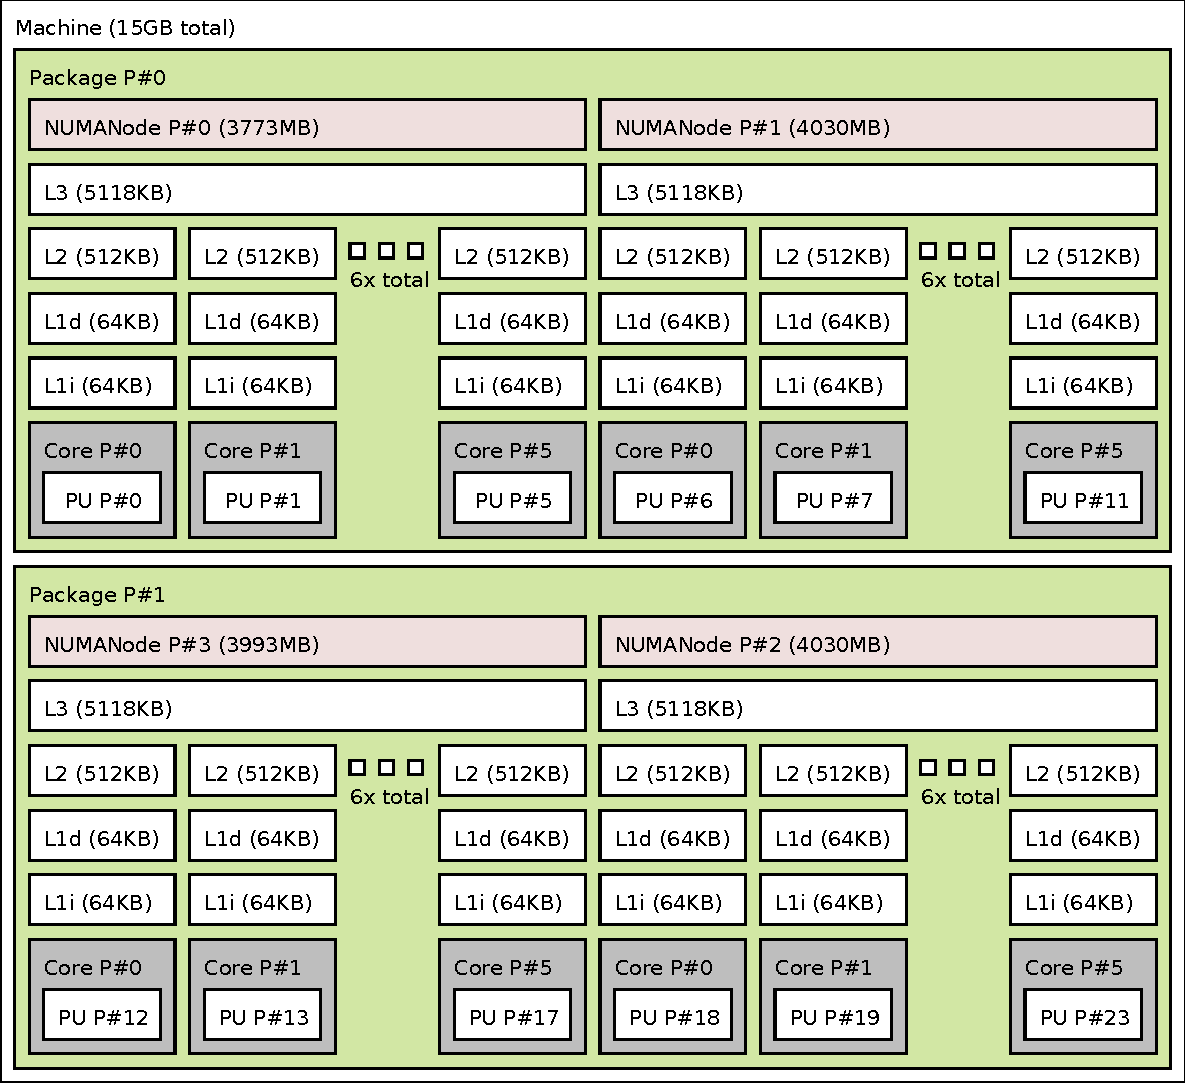
\includegraphics[width=0.8\textwidth]{Figures/paragon-topo.pdf}
	\linebreak
	\caption{Η τοπολογία του συστήματος Paragon.}
	\label{fig:paragon-topo}
\end{figure}


\section{Τοπολογία}
Η υλοποίηση των OpenMP places και OpenMP processor binding policies ελέγχθηκε για την ορθότητά της, δηλαδή  για το αν ικανοποιεί πλήρως τις προδιαγραφές του OpenMP, τόσο με ιδιόχειρα, όσο και με έτοιμα προγράμματα.   Τα έτοιμα προγράμματα ήταν μέρος ενός συνόλου προγραμμάτων ελέγχου ορθότητας τα οποία παρέχονται από τη βιβλιοθήκη \textit{GNU Offloading and Multi Processing Runtime Library} (libgomp) η οποία μεταξύ άλλων, υλοποιεί και τη διεπαφή προγραμματισμού εφαρμογών OpenMP που χρησιμοποιεί ο GCC.


\section{Barrier}
\label{sec:exp-barrier}
Η ορθότητα της υλοποίησης του tree barrier ελέγχθηκε για την ορθότητά της με προγράμματα ελέγχου από τη βιβλιοθήκη libgomp και την \textit{OpenMP Validation Suite V 3.0} \cite{wang2012openmp, ompvalsuite3}. Ο λόγος όμως που αναπτύχθηκε ο tree barrier ήταν οι μειωμένες επιδόσεις του υπάρχοντα barrier του OMPi σε συστήματα NUMA, οπότε αφού εξασφαλίστηκε η ορθότητα της υλοποίησης, θα εστιάσουμε στο ζήτημα των επιδόσεων με τη χρήση μετροπρογραμμάτων.

\subsection{EPCC OpenMP micro-benchmark suite}
Η \textit{EPCC OpenMP micro-benchmark suite} \cite{bull1999measuring} είναι ένα σύνολο μετροπρογραμμάτων (micro-benchmarks) τα οποία μετράνε το κόστος σε χρόνο (overhead) που απαιτείται για λειτουργίες όπως ο συγχρονισμός (π.χ. barrier, κλειδαριές), η \textit{χρονοδρομολόγηση βρόχου} (loop sceduling) και οι πράξεις πινάκων. Η πιο πρόσφατη έκδοση (3.1) υποστηρίζει μέχρι και τις λειτουργίες που προδιαγράφει το OpenMP 3.0.

Τα πειράματα που πραγματοποιήθηκαν επικεντρώθηκαν στη μέτρηση του overhead του barrier, όσο το πλήθος των κόμβων NUMA που χρησιμοποιούνται αυξάνεται. Με αυτό τον τρόπο ελέγχουμε κατά πόσο η εκάστοτε υλοποίηση barrier είναι κλιμακώσιμη. Οι υλοποιήσεις που συγκρίθηκαν είναι αυτές των μεταφραστών OMPi (κλασική και tree barrier), GCC, ICC και Clang. Η OpenMP processor binding policy παρέμεινε σταθερά στην τιμή \texttt{close}, ενώ σε κάθε OpenMP place τοποθετείται μόνο ένα νήμα OpenMP.


\subsubsection{Paragon}
Στα Σχήματα \ref{fig:bo-paragon-cores} και \ref{fig:bo-paragon-threads} φαίνεται το overhead του barrier κάθε μεταφραστή όταν χρησιμοποιούνται 1 έως 4 κόμβοι και ένα OpenMP νήμα ανά core ή H/W thread αντίστοιχα. Αυτό που παρατηρούμε, είναι ότι όταν \texttt{OMP\_PLACES="cores"} (Σχήμα \ref{fig:bo-paragon-cores}), για ένα κόμβο ο OMPi έχει το μικρότερο overhead, το οποίο όμως αυξάνει κατά πολύ για περισσότερους κόμβους. Στην περίπτωση που \texttt{OMP\_PLACES="threads"} (Σχήμα \ref{fig:bo-paragon-threads}), ο OMPi έχει εκθετική αύξηση του overhead για 2 ή περισσότερους κόμβους. Ο tree barrier και στις δύο περιπτώσεις έχει σαφώς καλύτερες επιδόσεις σε σχέση με τον κλασικό barrier του OMPi.

Εξαίρεση αποτελεί η χρήση ενός μόνο κόμβου, κατά την οποία o tree barrier είναι λίγο πιο αργός από τον κλασικό barrier. Κάτι τέτοιο όμως είναι αναμενόμενο καθώς γίνονται επιπλέον υπολογισμοί οι οποίοι δεν μπορούν να αποφευχθούν καθώς τα αποτελέσματά τους χρησιμοποιούνται για να αποφασιστεί αν θα χρησιμοποιηθεί ο tree barrier ή όχι. Για καλύτερη κατανόηση δείτε το Σχήμα \ref{fig:bo-paragon-ompionly}.

\begin{figure}[t]
	\centering
	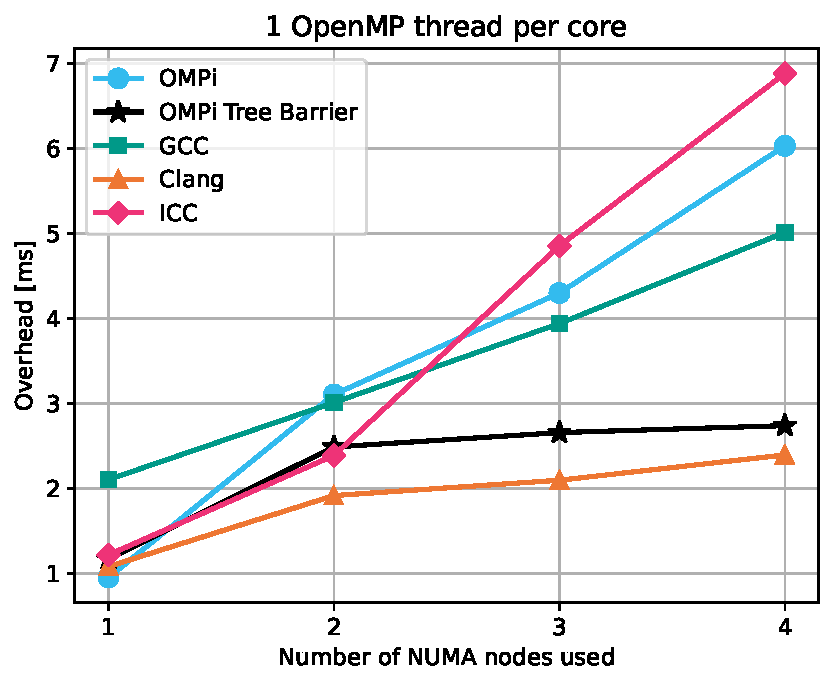
\includegraphics[width=0.7\textwidth]{Figures/epcc_20210823_175412/default-places_cores_close.pdf}
	\linebreak
	\caption{Barrier overhead στον Parade: OMP\_PLACES=cores.}
	\label{fig:bo-paragon-cores}
\end{figure}

\begin{figure}[t]
	\centering
	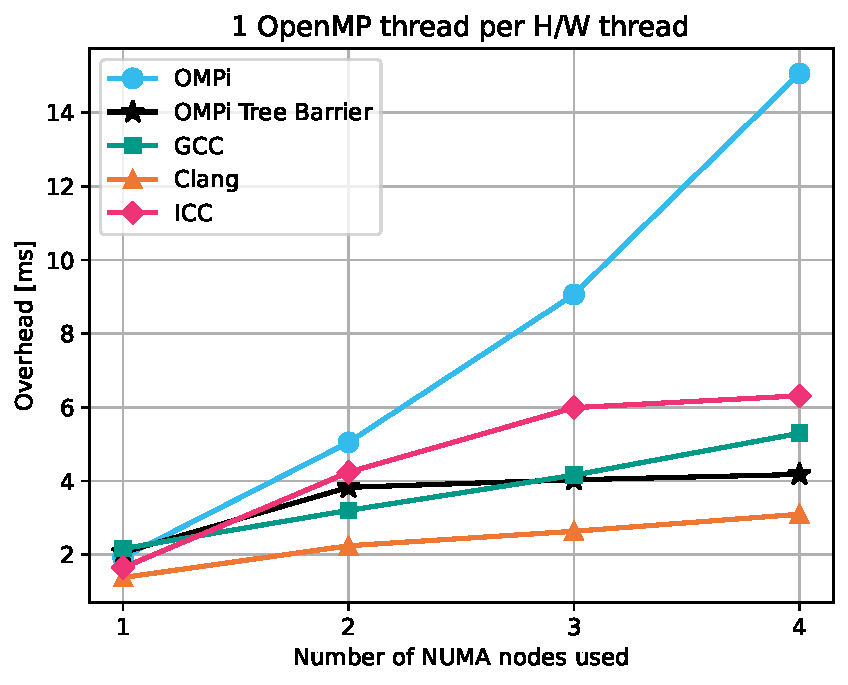
\includegraphics[width=0.7\textwidth]{Figures/epcc_20210823_175412/default-places_threads_close.pdf}
	\linebreak
	\caption{Barrier overhead στον Parade: OMP\_PLACES=threads.}
	\label{fig:bo-paragon-threads}
\end{figure}


\begin{figure}
    \centering
    \begin{minipage}{0.5\textwidth}
        \centering
        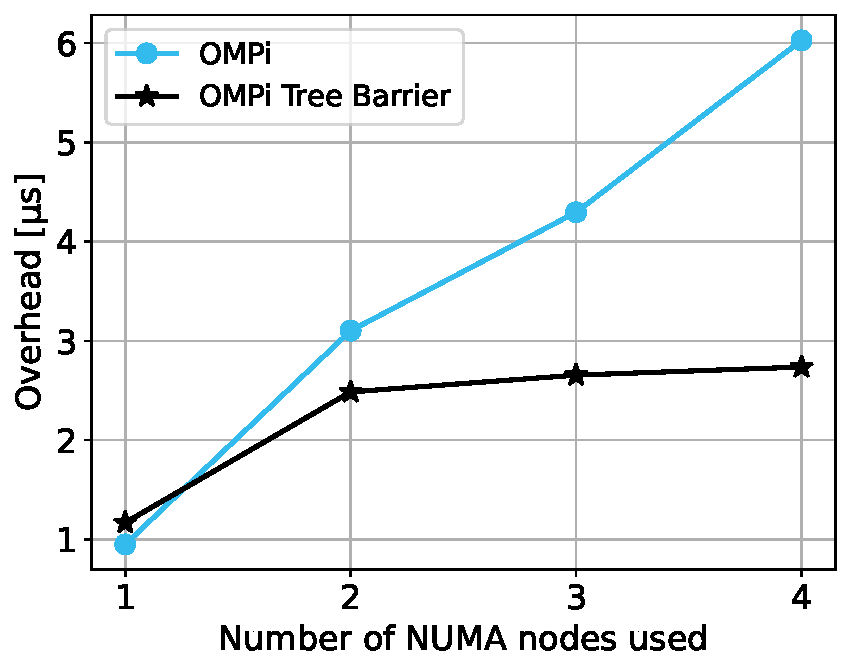
\includegraphics[width=1\textwidth]{Figures/epcc_20210823_175412/ompi_default-places_cores_close.pdf}
		\texttt{OMP\_PLACES=cores}
    \end{minipage}\hfill
    \begin{minipage}{0.5\textwidth}
        \centering
        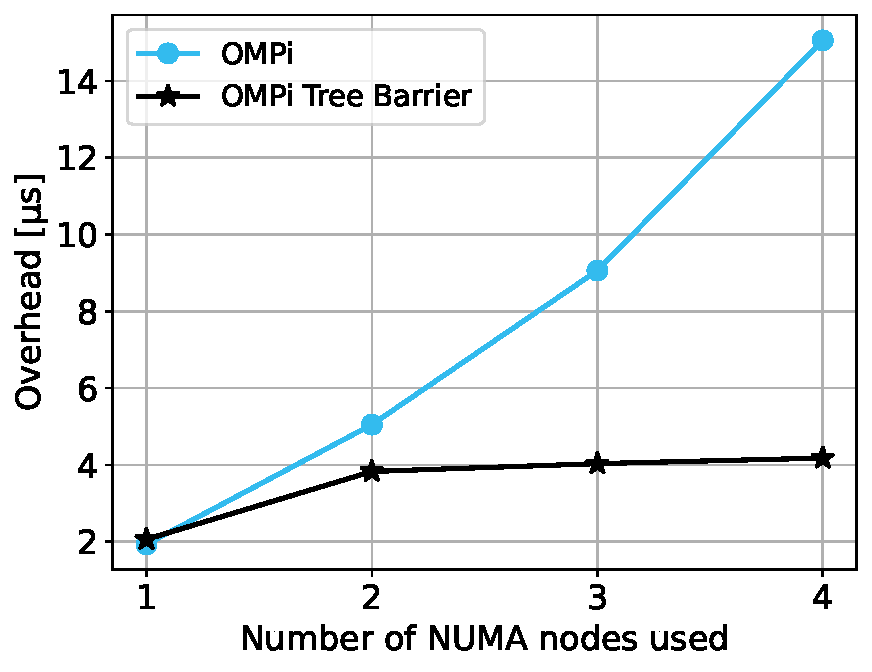
\includegraphics[width=1\textwidth]{Figures/epcc_20210823_175412/ompi_default-places_threads_close.pdf}
        \texttt{OMP\_PLACES=threads}
    \end{minipage}
    \caption{Barrier overhead στον Parade για τον κλασικό και tree barrier του OMPi.}
    \label{fig:bo-paragon-ompionly}
\end{figure}
